%___________________________ Q 4.2 ______________________________
\subsection{Show and describe the block diagram used to control the system. (1.5 pts)}
\vspace{10pt}

%%Write your answer here


The Simulink models employed for controlling the system are presented in Figure \ref{fig:simulink_models_no_integrator}. This figure illustrates three Simulink diagrams. The diagram in Figure \ref{fig:plant_interface} represents the plant interface, facilitating the interaction between the physical system and the control model. Specifically, sensor data and actuator signals are processed through this interface. Figure \ref{fig:state_estimator} depicts the state estimator, which is responsible for estimating the system states based on sensor inputs and control signals, utilizing a Kalman filter. Lastly, the state feedback controller, shown in Figure \ref{fig:controller_without_integrator}, is tasked with generating the control signals sent to the actuators. This controller does not incorporate integral action, which implies that a steady-state error is expected in the closed-loop system.

To address the steady-state error, a discrete-time integrator can be incorporated into the control system. This integrator processes the difference between the reference signal and the system output. The corresponding Simulink model is depicted in Figure \ref{fig:controler_with_integrator}. To mitigate the issue of integral windup, the integrator block is constrained with maximum and minimum limits, ensuring that the signal magnitude does not saturate the actuators even after the error has been corrected.
\begin{figure}[H]
    \centering
    \begin{subfigure}{0.47\textwidth}
        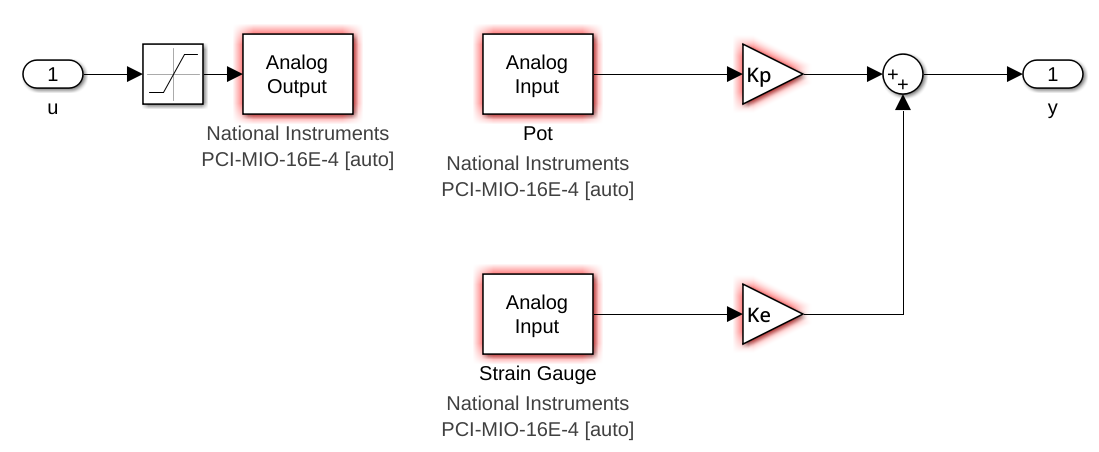
\includegraphics[width=\textwidth]{Figs/Simulink Models/Plant Interface.png}
        \caption{Plant interface}
        \label{fig:plant_interface}
    \end{subfigure}
    \hfill
    \begin{subfigure}{0.37\textwidth}
        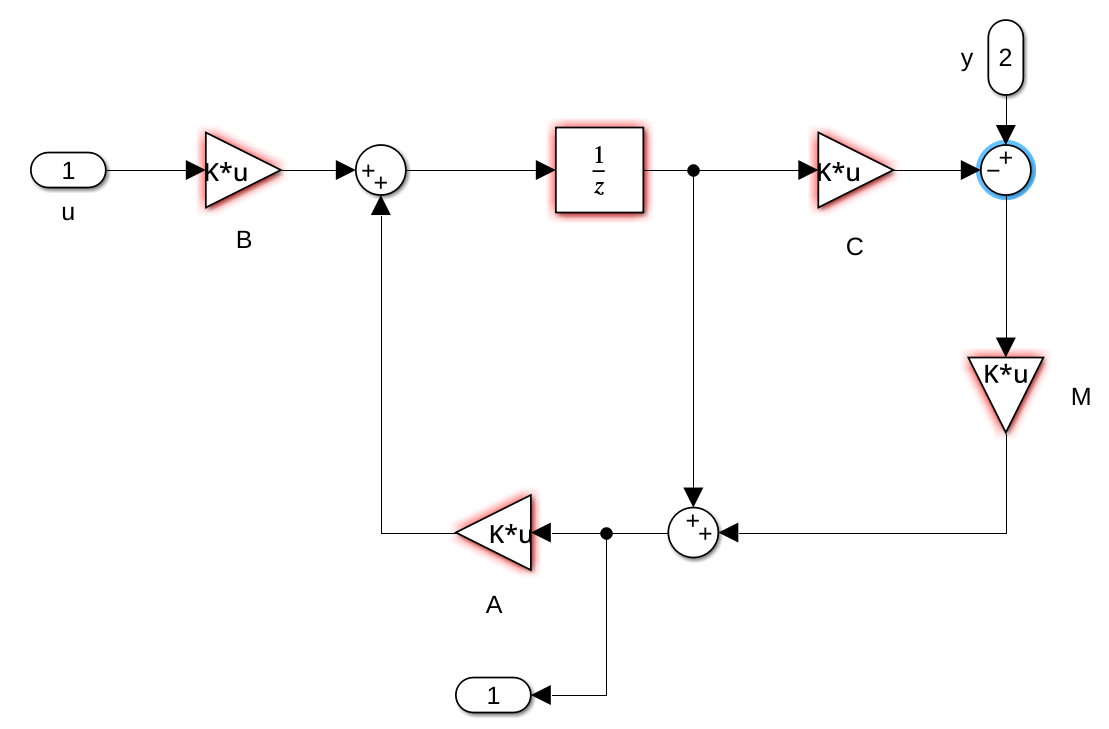
\includegraphics[width=\textwidth]{Figs/Simulink Models/State_Estimator.png}
        \caption{State Estimator}
        \label{fig:state_estimator}
    \end{subfigure}
    \begin{subfigure}{0.95\textwidth}
        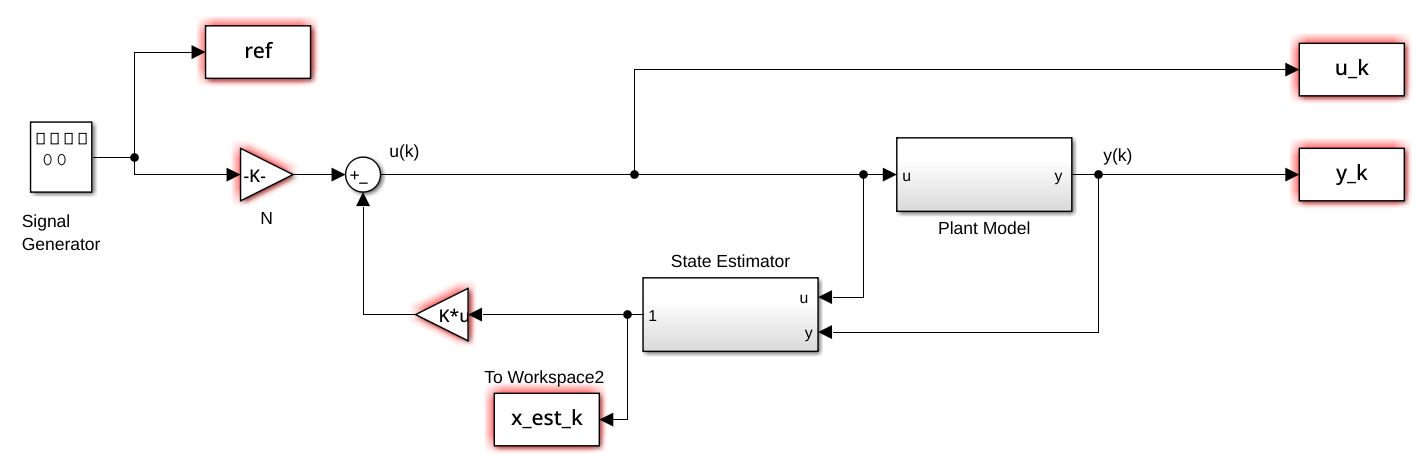
\includegraphics[width=0.9\textwidth]{Figs/Simulink Models/Controller_without_integrator.png}
        \caption{Controller without integrator}
        \label{fig:controller_without_integrator}
    \end{subfigure}
    \caption{Simulink models utilized for system control without integral action}
    \label{fig:simulink_models_no_integrator}
\end{figure}



\begin{figure}[H]
    \centering
    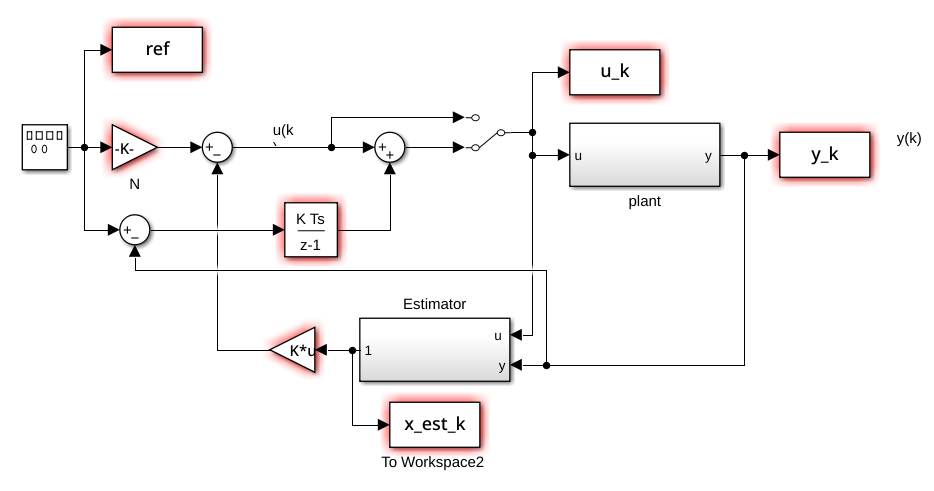
\includegraphics[width=0.7\textwidth]{Figs/Simulink Models/controller_with_integrator.png}
    \caption{Controller with integrator}
    \label{fig:controler_with_integrator}
\end{figure}
